\documentclass{standalone}
\usepackage{tikz}
\usepackage{pgfmath} % use to create randum numbers

\begin{document}
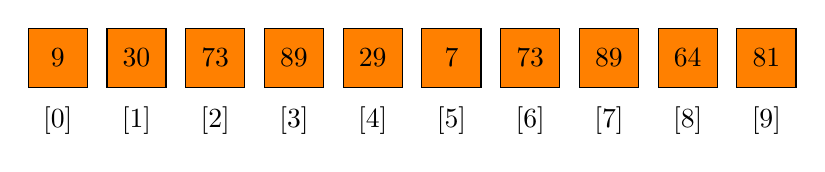
\begin{tikzpicture}[block/.style={rectangle, fill=orange, draw, minimum size=.75cm}]

% Create ten boxes
\foreach \i in {0,...,9} {
    % Create ten random numbers between i and 100 and store the value in variable `vara`
    \pgfmathparse{int(random(\i,100))}\let\vara=\pgfmathresult 

    % seeding ensures we have a random set of numbers everytime
    \pgfmathsetseed{\i}

    % Heres the labels
    \node[block] at (\i,0) {$\vara$};

    % and the subscripts
    \node[below] at (\i,-0.5) {[$\i$]};
}
\end{tikzpicture}
\end{document}